\documentclass[12pt]{ximera}
\title{Exam 1}
\begin{document}
\begin{abstract}
Exam 1, covering Sections 7.1--7.5: De Morgan's laws and Venn diagram shading,
inclusion-exclusion and independence from survey data, complements of unions, a
three-set Venn diagram of blood antigens, and a tree diagram for drawing two socks.
\end{abstract}
\maketitle

\section*{Exam 1}

Give your answers as exact fractions, decimals, or percentages; do not round unless
specifically asked to do so.

\begin{problem}
Assess whether each of the following claims is true or false.

\begin{prompt}
\textbf{(a)} Claim: the union of the complements of two sets can be equivalently
written as the complement of their intersection. That is, for sets $A$ and $B$,
\[ \olsi{A}\cup \olsi{B} = \olsi{A\cap B}. \]

\begin{multipleChoice}
\choice[correct]{True}
\choice{False}
\end{multipleChoice}

\begin{feedback}
True --- this is one of De Morgan's laws. To be outside the overlap of $A$ and $B$, you
must be missing from at least one of them, which is to say you are in $\olsi{A}$ or in
$\olsi{B}$.
\end{feedback}
\end{prompt}

\begin{prompt}
\textbf{(b)} Claim: the Venn diagram below shows the set
$\left(\olsi{A\cap B}\right)\cap C$.

\begin{center}
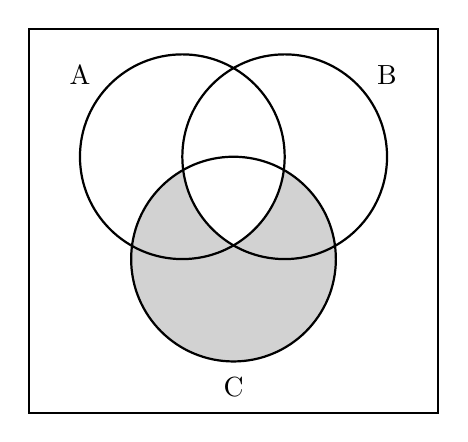
\begin{tikzpicture}[scale=1.3]
  \fill[gray!35] (0.5,-1) circle (1);
  \begin{scope}
    \clip (0,0) circle (1);
    \fill[white] (1,0) circle (1);
  \end{scope}
  \draw[thick] (0,0) circle (1) node at (-1,0.8) {A};
  \draw[thick] (1,0) circle (1) node at (2,0.8) {B};
  \draw[thick] (0.5,-1) circle (1) node at (0.5,-2.25) {C};
  \draw[thick] (-1.5,-2.5) rectangle (2.5,1.25);
\end{tikzpicture}
\end{center}

\begin{multipleChoice}
\choice[correct]{True}
\choice{False}
\end{multipleChoice}

\begin{feedback}
True. The shading is all of $C$ except the part that also lies in both $A$ and $B$.
Being outside $A\cap B$ is exactly what $\olsi{A\cap B}$ means, so the shaded region is
$\left(\olsi{A\cap B}\right)\cap C$.

Note the difference from $\olsi{A}\cap\olsi{B}\cap C$: that set would also remove the
parts of $C$ inside $A$ only or $B$ only, which here are still shaded.
\end{feedback}
\end{prompt}
\end{problem}

\begin{problem}
Suppose that in a survey of $70$ students, $50$ report they like wallabies and $35$
report they like axolotls; $20$ of the students report they like both.

\begin{prompt}
\textbf{(a)} How many students reported liking one or both of these animals?

$\answer{65}$ students.

\begin{feedback}
By inclusion-exclusion, $n(W\cup A)=50+35-20=65$.
\end{feedback}
\end{prompt}

\begin{prompt}
\textbf{(b)} What is the probability that a student who likes wallabies also likes
axolotls? Enter a fraction in lowest terms.

$\answer{2/5}$

\begin{feedback}
Of the $50$ wallaby-likers, $20$ also like axolotls:
$P(A\mid W)=\frac{20}{50}=\frac25$.
\end{feedback}
\end{prompt}

\begin{prompt}
\textbf{(c)} Recall that if $P(E\mid F)=P(E)$ then $E$ and $F$ are \emph{independent}.
Based on this data, are liking wallabies and liking axolotls independent events?

\begin{multipleChoice}
\choice{Yes}
\choice[correct]{No}
\end{multipleChoice}

\begin{feedback}
No. $P(A\mid W)=\frac25=0.4$, but overall $P(A)=\frac{35}{70}=0.5$. Since these differ,
knowing a student likes wallabies changes the probability they like axolotls.
\end{feedback}
\end{prompt}
\end{problem}

\begin{problem}
Suppose $\mathcal{U}=\set{0,1,2,3,4,5,6,7,8,9,10}$, with
\[
A= \set{0,2,4,6,8},\quad B= \set{0,3,6,9},\quad C= \set{1,2,3,4,5},\quad D= \set{7,8,9,10}.
\]
Which of the following are elements of the set $\olsi{A\cup C}$?

\begin{selectAll}
\choice{$0$}
\choice{$3$}
\choice{$6$}
\choice[correct]{$9$}
\choice[correct]{$10$}
\end{selectAll}

\begin{feedback}
$A\cup C=\set{0,1,2,3,4,5,6,8}$, so $\olsi{A\cup C}=\set{7,9,10}$. Of the listed
options, $9$ and $10$ belong to it.
\end{feedback}
\end{problem}

\begin{problem}
Human blood type is based on the presence of A antigens, B antigens, or Rh antigens.
The following data about blood type frequency was reported by the National Health
Service in 2018. Among blood donors,
\begin{itemize}
\item $75\%$ have Rh antigens;
\item $41\%$ have A antigens;
\item $13\%$ have B antigens;
\item $32\%$ have Rh and A antigens;
\item $10\%$ have Rh and B antigens;
\item $3\%$ have A and B antigens;
\item $2\%$ have all three of these antigens.
\end{itemize}

\begin{prompt}
\textbf{(a)} Fill in the seven regions of the Venn diagram, as percentages.

All three: $\answer{2}\%$

\smallskip
A and B only: $\answer{1}\%$ \qquad A and Rh only: $\answer{30}\%$ \qquad
B and Rh only: $\answer{8}\%$

\smallskip
A only: $\answer{8}\%$ \qquad B only: $\answer{2}\%$ \qquad Rh only: $\answer{35}\%$

\begin{hint}
Start at the center and work outward, subtracting the center from each two-antigen
figure first.
\end{hint}

\begin{feedback}
Center $2\%$. A and B only: $3-2=1\%$; A and Rh only: $32-2=30\%$; B and Rh only:
$10-2=8\%$. A only: $41-(1+30+2)=8\%$; B only: $13-(1+8+2)=2\%$; Rh only:
$75-(30+8+2)=35\%$.
\end{feedback}
\end{prompt}

\begin{prompt}
\textbf{(b)} What is the probability that a donor's blood contains none of these
antigens?

$\answer{14}\%$

\begin{feedback}
The seven regions total $2+1+30+8+8+2+35=86\%$, leaving $100-86=14\%$ outside all three
circles.
\end{feedback}
\end{prompt}

\begin{prompt}
\textbf{(c)} Based on this data, how many people would you expect to have all three of
these antigens in a group of $150$ people?

$\answer{3}$ people.

\begin{feedback}
$2\%$ of $150$ is $0.02\times 150=3$.
\end{feedback}
\end{prompt}

\begin{prompt}
\textbf{(d)} Based on this data, what are the odds that a random person has Rh
antigens? Reduce your answer.

The odds are $\answer{3}$ to $\answer{1}$.

\begin{feedback}
$75\%$ have Rh antigens and $25\%$ do not, so the odds are $75:25=3:1$.
\end{feedback}
\end{prompt}
\end{problem}

\begin{problem}
Suppose every morning, you draw two socks from a drawer containing $6$ red socks,
$4$ yellow socks, and $7$ blue socks, and whichever two socks you pull out are the two
you wear for the day. Enter every answer as a fraction in lowest terms.

\begin{prompt}
\textbf{(a, first sock)} $P(R)=\answer{6/17}$ \qquad $P(Y)=\answer{4/17}$ \qquad
$P(B)=\answer{7/17}$

\begin{feedback}
There are $6+4+7=17$ socks.
\end{feedback}
\end{prompt}

\begin{prompt}
\textbf{(a, second sock)} After one sock is removed, $16$ remain.

After red: \quad $P(R\mid R)=\answer{5/16}$ \quad $P(Y\mid R)=\answer{1/4}$ \quad
$P(B\mid R)=\answer{7/16}$

\smallskip
After yellow: \quad $P(R\mid Y)=\answer{3/8}$ \quad $P(Y\mid Y)=\answer{3/16}$ \quad
$P(B\mid Y)=\answer{7/16}$

\smallskip
After blue: \quad $P(R\mid B)=\answer{3/8}$ \quad $P(Y\mid B)=\answer{1/4}$ \quad
$P(B\mid B)=\answer{3/8}$

\begin{feedback}
Reduce the count of the first color by one and divide by $16$:
\begin{itemize}
\item after red: $5$ R, $4$ Y, $7$ B gives $\frac5{16}$, $\frac4{16}=\frac14$, $\frac7{16}$;
\item after yellow: $6$ R, $3$ Y, $7$ B gives $\frac6{16}=\frac38$, $\frac3{16}$, $\frac7{16}$;
\item after blue: $6$ R, $4$ Y, $6$ B gives $\frac38$, $\frac14$, $\frac38$.
\end{itemize}
\end{feedback}
\end{prompt}

\begin{prompt}
\textbf{(b)} Multiply along each path to find the probability of each outcome.

$P(RR)=\answer{15/136}$ \quad $P(RY)=\answer{3/34}$ \quad $P(RB)=\answer{21/136}$

\smallskip
$P(YR)=\answer{3/34}$ \quad $P(YY)=\answer{3/68}$ \quad $P(YB)=\answer{7/68}$

\smallskip
$P(BR)=\answer{21/136}$ \quad $P(BY)=\answer{7/68}$ \quad $P(BB)=\answer{21/136}$

\begin{feedback}
Every path has denominator $17\cdot 16=272$. The numerators are
\[
\begin{array}{lll}
RR: 6\cdot 5=30 & RY: 6\cdot 4=24 & RB: 6\cdot 7=42\\
YR: 4\cdot 6=24 & YY: 4\cdot 3=12 & YB: 4\cdot 7=28\\
BR: 7\cdot 6=42 & BY: 7\cdot 4=28 & BB: 7\cdot 6=42
\end{array}
\]
which total $272$. \checkmark Reducing, for example, $\frac{30}{272}=\frac{15}{136}$.
\end{feedback}
\end{prompt}

\begin{prompt}
\textbf{(c)} What is the probability that you draw matching socks?

$\answer{21/68}$

\begin{feedback}
Add the three matching outcomes:
\[
\frac{30+12+42}{272}=\frac{84}{272}=\frac{21}{68}\approx 0.309.
\]
\end{feedback}
\end{prompt}
\end{problem}

\end{document}
